\section{TPU explained in depth}
\label{sec:hard-tpu}
% cite page https://qengineering.eu/google-corals-tpu-explained.html
The Google Coral has a TPU on board which speeds up the tensor calculations
enormously. These tensor calculations are used in deep learning and neural
networks. \hfill \break 
The Google Coral Dev board use an ASIC made by the Google team called the Edge 
TPU. It is a much lighter version of the well-known TPUs used in Google's 
datacenter. \hfill \break
It also consumes very little power, so it is ideal for small embedded systems. 
Nevertheless, the similarities in applied technology are significant.\cite{TPU:explained} 
%
\subsection{Neural Node}
\label{ssec:hard-neural-node}
Neural networks used in deep learning consists of many neural nodes. They are
all connected together in a defined way. The way these nodes are wired is
called the topology of the network. This topology determines the function the
network performs. See this list for a selection of several types of deep
learning networks. Each node has always three basic components. 
A multiplier multiplies all the inputs with their respective so-called weight,
the synapses. An adder who accumulates all the individual multiplications. 
And an activation function that shapes the output given the addition. A
schematic view below (\ref{fig:neuron}).\hfill \break
%
\begin{figure}[htb]
	\centering
	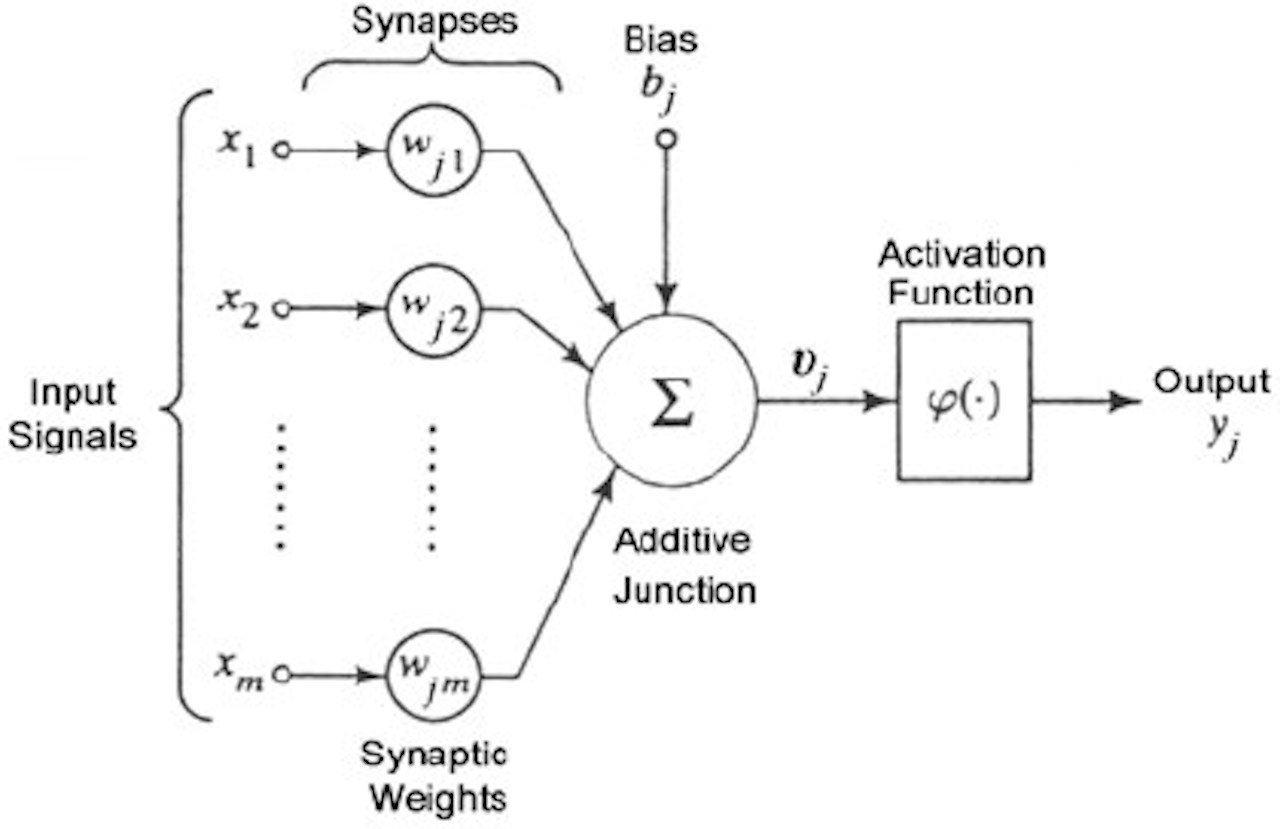
\includegraphics[width=0.70\textwidth]{sinapse.jpg}
	\captionsource{Artificial Neuron models and its parts.}{Adapted from Haykin (1994)}
	\label{fig:neuron}
\end{figure}
%
\newpage
\noindent The formula can be written as follows \eqref{eq:neuron}.
\begin{equation}
\label{eq:neuron}
	y_{i} = \phi \, \left(\sum_{i=1}^{n} w_{ij}\cdot x_{i} \right)
\end{equation}
%
Deep neural network is consist of millions of neural nodes distribute over many
layers; despite the simplicity of the operation, only on multiplication and one
addition, require long compute time to obtain a result. keep in mind that for
training a network requires many epochs. In other words, the main problem is
time. The algorithms is well suited for parallel execution. Although
distributing the algorithm over the processes and threads can be an option
actually provides disappoint results for the presence of bottlenecks due to
architecture general purpose. On the other hand use of Graphical Processing
Unit, the GPU on video card designed for efficient manipulation memory. Their
highly parallel structure make them more efficient respect CPU especially for
algorithms that process large blocks of data in parallel. The best choice is the
use of the Tensor Processing Unit, the TPU. This device has been specially
designed for the above neural node algorithm.
%
\subsection{The adder}
\label{ssec:hard-adder}
Generally a strategy adopted when software is tool slow is modify the hardware
to reach the better achievements.
The structure inside TPU is realized by three main components derived from 
neural node, then keeping in mind the scheme in figure (\ref{fig:neuron}): the 
\textbf{multiplier}, the \textbf{adder} and the \textbf{activation function} 
must be included in the hardware.
Start with analysing the diagram of the 4-bit adder realized in figure
(\ref{fig:4-bit-adder}).
Where: \texttt{A} and \texttt{B} are the inputs. If the output overflows 
\texttt{C4} the carry out is set. \texttt{C0} is the carry-in of a previous 
phase.\cite{TPU:explained}
%
\begin{figure}[!h]
	\centering
	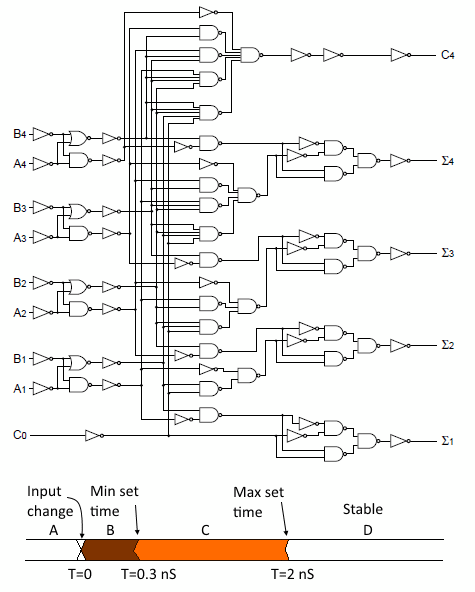
\includegraphics[width=0.75\textwidth]{Adder1.png}
	\captionsource{4-bit adder}{\href{https://qengineering.eu/google-corals-tpu-explained.html}{Q-engineering}}
	\label{fig:4-bit-adder}
\end{figure}
%
Signals \texttt{A} and \texttt{B} propagate through the circuit and generate the
result \texttt{A + B}. Changing one of them alters almost immediately the
output. This happens extremely very fast, within a few nanoseconds. This
propagation time depends on the number of digital ports whose output changes.
The propagation time is therefore not fixed, but lies between two limits, a
minimum and a maximum time, see diagram at the bottom of the drawing
(\ref{fig:4-bit-adder}). By the way, al mentioned times are illustrative and
have no relationship to any device.\cite{TPU:explained}
%
\newpage
\subsection{Pipeline}
\label{ssec:hard-pipeline}
Consider the example where: the propagation time of one adder is $2 \,
\si{\nano\second}$, therefore the maximum clock rate can be $500
\,\si{\mega\hertz}$. Taking into account that a neural node can have many
inputs, also hundreds, that must be accumulated this affect the propagation time
that increase dramatically. This implies that the last adder in the chain must
be attend all intermediate result before its output becomes stable. 
If we consider a chain of 250 input each of one with $2\, \si{\nano\second}$
delay, we obtain total time of $500 \,\si{\nano\second}$ waiting. \\ 
Consequently clock results extremely slow $2\,\si{\mega\hertz}$, then solution
adopted is structured pipeline where between each adder is inserted a memory
element that keep keeps the result stable for the next adder. 
As show in figure (\ref{fig:4-bit-adder-register}). \hfill \break
%
\begin{figure}[!h]
	\centering
	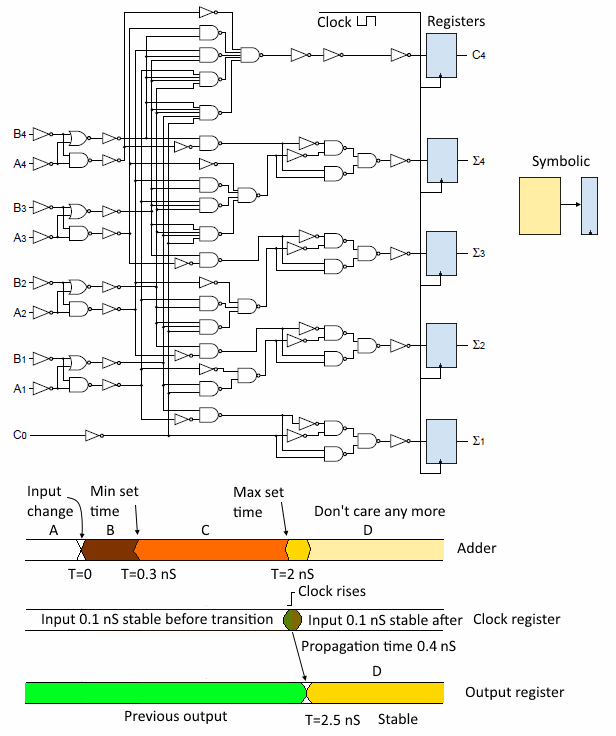
\includegraphics[width=0.75\textwidth]{AdderReg10.png}
	\captionsource{4 bit adder with register}{\href{https://qengineering.eu/google-corals-tpu-explained.html}{Q-engineering}}
	\label{fig:4-bit-adder-register}
\end{figure}
%
\break The output of the registers is updated at the rising edge of the clock
signal. That is the only time the output can change. When the clock signal is
high or low, the inputs cannot manipulate the output, then it remains stable. 
Just before the clock rises, the input must be stable for a minimum time, also
just after the rise time. In contrast to the previous example, now consider a
delay of $0.1 \,\si{\nano\second}$ and adding the register's propagation time of
$(0.4 \,\si{\nano\second})$, the total propagation reach for a new stable signal
is now $2.5 \si{\nano\second}$, which results increasing up to clock speed of
$400 \,\si{\mega\hertz}$. Observable in figure (\ref{fig:pipe}).
%
\begin{figure}[htb]
	\centering
	\includegraphics[width=0.60\textwidth]{pipe10.png}
	\captionsource{Digital pipeline.}{\href{https://qengineering.eu/google-corals-tpu-explained.html}{Q-engineering}}
	\label{fig:pipe}
\end{figure}
%
%
Taking into account the table in figure \ref{fig:pipe}, each color represents a
value. After four clock cycles, the value at the input has propagated through
the network and appears at the output.	Because the registers are updated
simultaneously a new input is accepted every $2.5 \,\si{\nano\second}$.	The
propagation time has been restored. The time it takes to travel through the
whole pipeline is called latency time and is $10 \,\si{\nano\second}$ in the
above diagram $(4 \times 2.5 \,\si{\nano\second}$). Every digital component is
built on large pipelines which guarantee the required speed.\cite{TPU:explained}
 
%
\subsection{The mul-add cell}
\label{ssec:The-mul-add-cell} 
The input signal of every neural node has effect on final result. This gives a
simple multiplication for an input mediate by a weight value. The operation of
multiplication can be implemented with same logic of an adder, then are
necessary more gates. 
Remembering that the neural node has multiplied his value for weight value. 
Thus the representation assume the scheme in figure
(\ref{fig:mul-add-register}).\hfill \break
%
\begin{figure}[htb]
	\centering
	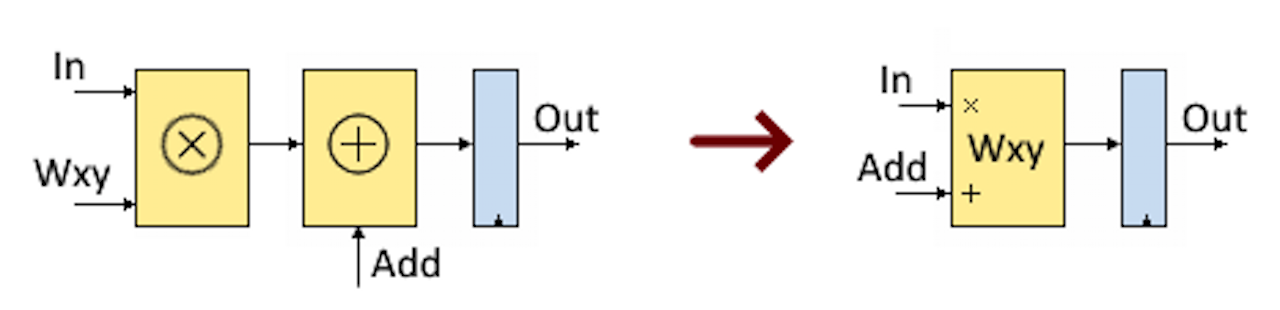
\includegraphics[width=0.65\textwidth]{MulAddReg10.png}
	\captionsource{Mul-Add register.}{\href{https://qengineering.eu/google-corals-tpu-explained.html}{Q-engineering}}
	\label{fig:mul-add-register}
\end{figure}
%
%
%\break For the sake of simplicity, no additional propagation time fixing registers have
%been added. With the formula of the neural node in mind, it is now relatively
%easy to design such a neuron with a few mul-add cells. Below the schematic for a
%three input neuron.
%
\begin{figure}[htb]
	\centering
	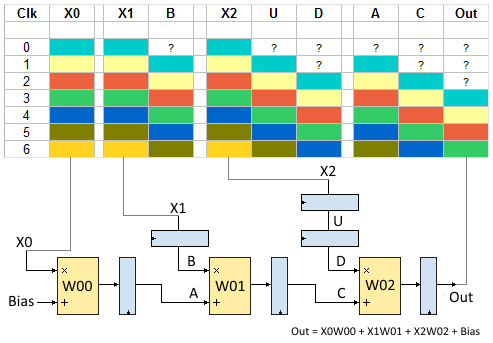
\includegraphics[width=0.75\textwidth]{Neuron.png}
	\captionsource{Schematic for a
three input neuron.}{\href{https://qengineering.eu/google-corals-tpu-explained.html}{Q-engineering}}
	\label{fig:3-input-neuron}
\end{figure}
%
%
\newline
Are necessary many important clarifications about the input registers
\texttt{X1} and \texttt{X2} displayed in figure (\ref{fig:3-input-neuron}). They
generate a delay line in the \emph{mul-add} chain, thus can permit to correct
synchronize. Considering the second cell \emph{mul-add} who sum the output from
previous cell (signal \texttt{A}) retarded by one clock cycle. Consequently also
the multiplication between the value in register \texttt{X1} and weight value
must be delayed the same amount of time. The schema reported in figure
(\ref{fig:3-input-neuron}) shows for each colour that represent the vector of
input \texttt{$[X0, X1, X2]$} while the input \texttt{A} and \texttt{B},
represented by lines straight, maintains always same colour. This means that
they appear simultaneous, i.e. are synchronised. The same must be valid for
input \texttt{C} and \texttt{D}.
%
\subsection{Systolic array}
\label{ssec:hard-systolic-array}
Starting from structure, just examined, is quite easy extend it to other
neurons, taking into account that every single input is connected with all
neurons in the next layer, as shows in figure
(\ref{fig:systolic-array-edge-tpu}).
%
\begin{figure}[htb]
	\centering
	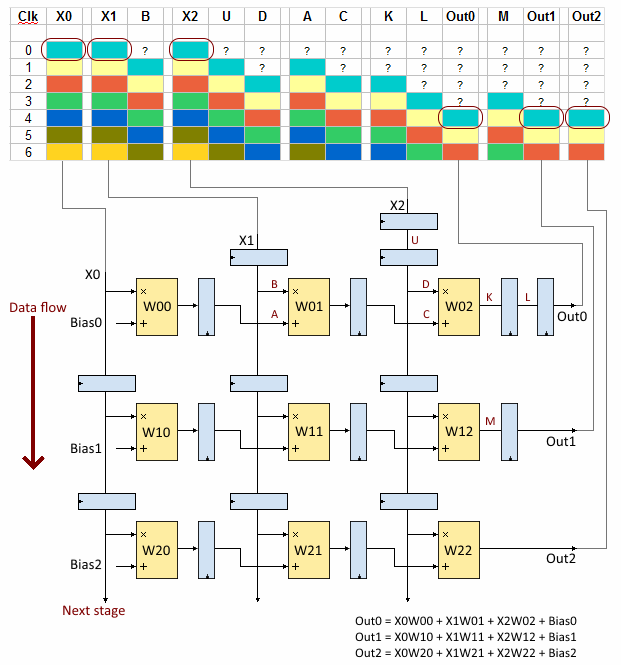
\includegraphics[width=0.75\textwidth]{Systolic-Array.png}
	\captionsource{Systolic Array Edge TPU.}{\href{https://qengineering.eu/google-corals-tpu-explained.html}{Q-engineering}}
	\label{fig:systolic-array-edge-tpu}
\end{figure}
%
%
The adoption of this solution, called systolic array, permits to have an
increment of speed in parallel calculation. 
Since the propagation time remains unchanged for an spread of systolic array in
depth or width, while only the latency time grows up this represent the solution
widely used for neural network hardware.
%
%The sizes of the systolic array in the Edge TPU are not known yet. The first TPU
%Google uses in its datacenter contains 256 x 256 \emph{mul-add} cells. Running at 700
%MHz it can theoretical performs 256 x 256 x 700.000.000 = 46 trillion \emph{mul-adds}
%per second. Or if you look to individual operations 92 trillion (92 TOPS).
%However, this impressive figure is purely theoretical. In practice, there are
%some factors that slow performance.
%
%The systolic array is made up of hardware. This means that it has fixed
%dimensions. Therefore, the input and output vectors also have fixed dimensions.
%However, the numbers of neurons per layer are determined by the design and are
%certainly not constant. If the number is smaller than the size of the array, it
%is, of course, possible to expand an input vector with leading zeros, so that
%the dimension equals the array size. The same technique can be applied to an
%oversized output vector.
%
%If the input vector contains more elements than the width of the systolic array,
%the entire arithmetic calculation must be performed in more than one call. To
%this end, the input vector is cut into a series of smaller vectors that match
%the width of the series. They are then processed one after the other. The
%intermediate results must be stored in a buffer. These values must be added
%after completion of all the systolic calls. Note that not only the input vector
%is split into smaller parts, but all weights used in the multiplication must be
%updated according to the formula's processing section. This may require a
%massive memory transfer. Below an example of a systolic array with only four
%inputs processing a vector of size 12.
%
%
%
%Looking at Google's schematic overview of the TPU, these output buffers and
%accumulators are drawn at the bottom. (In their diagram, the output is at the
%bottom instead of the right as on our drawing).
%Google TPU detail
%
% 
%Buffers have also been placed on the input vector side in the diagram above.
%They act as a first-in-first-out buffer, a FIFO. This guarantees continuous
%input of the systolic array with input values. It may also have some rotating
%operations, which increases the performance of CNN networks. It is unclear
%whether Google uses this method here. 
%
%
\subsection{Activation unit}
\label{ssec:activation-unit}
Once the output is available, it is sent to the activation unit. This module
within the Edge TPU applies the activation function to the output. It is
hardwired. In other words, you cannot alter the function, it works like a ROM.
Probably it is a ReLU function as it is nowadays the most used activation
function and it is very easy to implement in hardware.\cite{TPU:explained}
%
%
% TPU versus Edge TPU. The Google's Edge TPU is a much smaller device than the
% TPUs that Google uses in its data centers. Below the PCB with the original TPU
% and the Edge TPU on the same scale. TPU vs Edge TPU It is obvious that such a
% small device cannot have the same functions as its much larger ancestor. The
% floor plan on the die does not allow this to happen. Nor can the systolic
% array have the $256 \times 256$ dimension as in the original TPU. Google has
% so far not revealed the measures in the Edge, but a well-founded estimate is
% $64 \times 64$ with a clock of $480 \si{\mega\hertz}$, resulting in 4 TOPS.
% Memory is also an issue. In the original chip, it takes around $29\%$ of the
% total floor plan. It is impossible that the same amount can be found on the
% Edge TPU die. Moreover, the chip is very energy efficient. It requires no
% cooling. This means that almost certainly all the buffering is outside the
% chip. It leaves only a simple transfer of input vectors, output vectors and
% weights to the chip.	
% Practice.

